\documentclass[10pt]{article}
\usepackage{indentfirst}
\usepackage[margin=0.5in]{geometry}
\usepackage{multicol}
\usepackage{commath}
\setlength{\columnsep}{0.3in}
\usepackage{graphicx}

\usepackage{caption}
\usepackage{subcaption}



\begin{document}

\begin{center}

\LARGE The Relationship between Masers and AGN in X-Ray and Optical Spectra\\
\large Andrew Nutter\\
\small Department of Physics and Astronomy, James Madison University, Harrisonburg, VA 22807, USA\\
\small \today

\end{center}

\begin{abstract}
\noindent abstract abstract abstract abstract abstract abstract abstract abstract abstract abstract abstract abstract abstract abstract abstract abstract abstract abstract abstract abstract abstract abstract abstract abstract abstract abstract abstract abstract abstract abstract abstract abstract abstract abstract abstract abstract abstract abstract abstract abstract abstract abstract abstract abstract abstract abstract abstract abstract abstract abstract abstract abstract abstract abstract abstract abstract abstract abstract abstract abstract abstract abstract abstract abstract abstract abstract abstract abstract abstract abstract abstract abstract abstract abstract abstract abstract abstract abstract abstract abstract abstract abstract abstract abstract abstract abstract abstract abstract abstract abstract abstract abstract abstract abstract abstract abstract 

\end{abstract}

\begin{multicols}{2}
\section{Introduction}
introduction introduction introduction introduction introduction introduction introduction introduction introduction introduction introduction introduction introduction introduction introduction introduction introduction introduction introduction introduction introduction introduction introduction introduction introduction introduction introduction introduction introduction introduction introduction introduction introduction introduction introduction introduction introduction introduction introduction introduction introduction introduction introduction introduction 
introduction introduction introduction introduction introduction introduction introduction introduction introduction introduction introduction introduction introduction introduction introduction introduction introduction introduction introduction introduction introduction introduction 
\section{Methods}\label{methods}
The list of maser detections and the control group of surveyed non-masers were crossmatched against X-Ray and Optical telescope survey data to learn more about what masers can tell us about AGN. First an appropriate control group had to be established. Then, appropriate crossmatch radii had to be chosen. Finally, this data was collected so that information could be extrapolated from detection rates and further associated data such as flux.

\subsection{Building a Maser Control Sample}\label{control}
The Megamaser Cosmology Project has provided a list of all 4,464 (as of the spring of 2013) surveyed galaxies\cite{surv}. This list includes all galaxies surveyed; as such it includes many duplicates as well as most of the masers. In order to effectively gather statistical data it was necessary to establish an appropriate control group, requiring removal of any duplicates as well as all detected masers.

The first steps taken were to filter out all duplicates and then to crossmatch with the maser list in order to identify and then remove all maser detections. Using AWK code in the UNIX command line, the duplicates were removed first by name, resulting in 3,617 results, then by position. The galaxies were sorted according to right ascension, so duplicates were removed by eliminating consecutive galaxies within a declination of 10", resulting in 3,485 results.

Crossmatching this in SQL against the list of all masers with an angular separation of up to 10" resulted in 128 matches, as opposed to the size of the maser list, which was 151. Presumably, the all-surveyed results should include each of the 151 masers. The only way to increase the results to 151 matches was by an increase in radius to 36". Of the new 23 results, some were not actual matches but different galaxies entirely. Filtering out the 128 results from the list of 3,485 unique objects using SQL yielded 3,357 unique maser non-detections. Crossmatching this against the SDSS with an angular separation radius of 10" resulted in 2,181 matches.

Because not all maser detections were found in the all-surveyed sample, further steps were required to confirm an accurate control group. In order to accomplish this, the prior steps were done in reverse order to ensure a comprehensive view comparing the maser list with the entire all-surveyed sample. The list of 4,464 was matched directly against the 151 detections at 10" and 6' resulting in 782 and 807 matches respectively. The margin of 25 additional results were each individually interpreted by hand to decide whether or not they should be in the control group.Various internet resources were used such as the SDSS Navigator\cite{navigator} in order to confirm whether or not each object was a maser detection, a unique non-detection, or a duplicate. Table 1 displays this information.

The marked galaxies* were determined to be unique from the maser list. Those 8 galaxies were kept in the control by removing them from the list of 807 used for filtering. The unmarked galaxies were determined to be maser matches and were left in the filter list. The remaining filter filter list contained 799 objects. It turns out that these 799 represented 120 of the maser detections from the maser list. It was later discovered that the 128 found earlier did include some duplicates, and actually represented 119 maser detections. This inclusion of new items to the filter list helped remove maser detections that were missed by the previous filter. These 799 results were filtered from the all-surveyed list and then duplicates were removed from that list. The resulting maser control list, confirmed to have excluded all maser detections and duplicates within 10", contained 3,339 unique galaxies.

\end{multicols}
\begin {table}
\caption {Radii Gap Annulus} \label{radiigap}
\begin{center}
{\footnotesize \begin{tabular} {|p{4cm}|p{1.2cm}|p{1.2cm}|p{0.8cm}|p{6.7cm}|}
  \hline
\large Name & \large RA & \large DEC & \large Velo & \large Treatment \\
 \hline 
 \hline
*005420-233309 & 13.5854 & -23.5525 & 9680 & Keep, unique from NGC235A \\ \hline
0437170 & 69.3208 & 66.62833 & 770 & Exclude, J0437+6637 duplicate \\ \hline
0508212 & 77.0883 & 17.3689 & 5049 & Ambiguous so exclude because 19.9">10" \\ \hline
0719308+5921184 & 109.879 & 59.3551 & 3258 & Exclude, UGC3789 duplicate \\ \hline
*091958+264455 & 139.992 & 26.7485 & 7898 & Keep, unique from IC485 \\ \hline
*120210+351355 & 180.543 & 35.2319 & 10077 & Keep, Unique from J1202+3519 \\ \hline
*2MASXJ11092911+2841293 & 167.371 & 28.6914 & 9847 & Keep, Unique from J1103-0052 \\ \hline
*IC486 & 120.088 & 26.6135 & 8062 & Keep, unique from IC485 \\ \hline
IC694 & 172.072 & 58.5507 & 3064 & Exclude, they are arp299 \\ \hline
NGC3690A & 172.081 & 58.5371 & 3064 & Exclude, they are arp299 \\ \hline
NGC3690B & 172.102 & 58.534 & 3064 & Exclude, they are arp299 \\ \hline
NGC4151half & 182.598 & 39.3804 & 995 & Exclude, NGC4151 dupe see 995 \\ \hline
*NGC4156 & 182.707 & 39.4728 & 6755 & Keep, unique from NGC4151 \\ \hline
NGC4258N & 184.733 & 47.3082 & 466 & Exclude, NGC4258 duplicates \\ \hline
NGC4258NN & 184.731 & 47.3109 & 466 & Exclude, NGC4258 duplicates \\ \hline
NGC4258NNN & 184.731 & 47.3137 & 466 & Exclude, NGC4258 duplicates \\ \hline
NGC4922B & 195.316 & 29.3061 & 7056 & Exclude, NGC4922/130125+291849 duplicate \\ \hline
NGC520a	 & 21.1437 & 3.79497 & 2266 & Exclude, 520 duplicates \\ \hline
NGC520b	 & 21.145 & 3.78969 & 2266 & Exclude, 520 duplicates \\ \hline
NGC520m1 & 21.1451 & 3.78408 & 2266 & Exclude, 520 duplicates \\ \hline
NGC520m2 & 21.145 & 3.79525 & 2266 & Exclude, 520 duplicates \\ \hline
NGC520m3 & 21.1395 & 3.78972 & 2266 & Exclude, 520 duplicates \\ \hline
NGC520m4 & 21.1505 & 3.78975 & 2266 & Exclude, 520 duplicates \\ \hline
*NGC5256A & 204.587 & 48.242 & 8211 & Keep, unique from NGC5256 \\ \hline
*notMrk78 & 115.674 & 65.1436 & 11137 & Keep, unique from Mrk78 \\
  \hline
\end{tabular}}
\end{center}
\end {table}
\begin{multicols}{2}

\subsection{Crossmatching Against Catalogs}\label{match}
The maser and control groups were crossmatched against the Chandra Source Catalog (CSC), ROSAT All Sky Survey (RASS), Swift-BAT, Integral, Sloan Digital Sky Survey data release 9 (SDSS DR9), and 2XMMi-DR3. First an angular search radius had to be chosen for each catalog's crossmatch based on its precision. Next, the crossmatches were performed and detection rates were calculated.
\subsubsection{Selecting Angular Separation}\label{angle}
In order to determine the best angular separation radius for the CSC and the RASS Bright Source Catalog (RBSC), numerous crossmatches were made against a combination table containing both the control list and the list of all maser detections. The RBSC was matched at 10 arcseconds to 70" in increments of 10" and a histogram was formed from the number of results within each annulus described as the space between two successive radii. The same was done for CSC from 1" to 7" in increments of 1".

RASS has previously been compared to the TYCHO catalog (precision of 1") in a similar manner\cite{voges}. The number of mismatches per annulus has been shown by this study and others\cite{parejko} to be a linear relationship between random matches and angular separation. Voges' findings showed that by 40", reliable matches cease be found. Their results indicated that 90\% of RBSC sources are found within 25".

The RBSC histogram shown in Figure 1, displaying the number of matches per annulus, indicates a high incidence of matches until 10" at 115, with 47 matches between 10" and 20". This accounts for 87\% of all detections found until 70". From 20" to 30", there were 13 more matches which brings it up to 94\% of all matches. 

There is not enough data to determine the slope of the line describing the number of mismatches within each successive annulus. Likewise, any percentage of total matches that are mismatches is also impossible to calculate precisely. However, because it is known that the number of mismatches per annulus increases linearly with angular separation, it is still possible to interpret how its significance will vary.

A ratio can be described---the "angle-to-margin" ratio---of a given angular radius to the number of matches in the annulus since the previous radius. Another ratio can be described---the "mismatch-to-margin" ratio---which is the ratio of mismatches in that annulus to total marginal matches in the same annulus; in other words, the percentage that are mismatches. Because the number of mismatches in each annulus increases linearly with angular radius, the rate at which the mismatch-to-margin ratio changes is the same at every point as the rate at which the angle-to-margin ratio changes. While we still cannot find each individual mismatch-to-margin ration, this relationship allows us to extrapolate valuable information about its rate of change because we can calculate each individual angle-to-margin ratio.

This rate of change is calculated sequentially as the factor by which the ratio changes, and has been labelled the Percentage Increase Factor (PIF) value. Each PIF value is calculated by dividing the angle-to-margin ratio from one radius by the angle-to-margin ratio from the previous radius. Because the formula relies on two successive annulus match counts leading up to the current angular radius, the first angular radius that a PIF value can be calculated for is 20" for RBSC and 2" for CSC. This describes the rate of change of percentage of mismatches, and as such presents a curve that roughly depicts the derivative of the percentage of mismatches per margin. 

\begin{equation}
PIF = \frac{\dfrac{\phi_n}{c_n}}{\dfrac{\phi_{n-1}}{c_{n-1}}} = \frac{\phi_n\times c_{n-1}}{\phi_{n-1}\times c_n}\\
\end{equation}

\indent \indent \indent $\phi_n =$ angular radius in question\\
\indent \indent \indent $\phi_{n-1} =$ previous angular radius\\
\indent \indent \indent $c_n =$ count within this annulus\\
\indent \indent \indent $c_{n-1} =$ count within previous annulus\\

Graphing these results for each angular radius shows that these values peak somewhere between 20" and 30", presumably near 25". The peak of the PIF function represents the highest rate of change in the percent of mismatches, an inflection point on the curve of the percent of randoms per annulus. This can be assumed to be a peak because until this point, the marginal matches curve has just peaked and its slope is becoming more and more negative. This suggests that the percent of matches that are mismatches is increasing more and more quickly, and likewise that PIF values are increasing.

All matches before the peak (or the inflection point on a percent curve) can be said to be dominated by true matches, as they fit closely to the Rayleigh distribution as described by Voges et al. Matches after the peak asymptotically approach the line describing random matches. As such, everything after the peak represents a shift in influence where the number of matches per annulus is dominated by mismatches. Based on this peak around 25", the similar curve represented by Voges' data, and their suggestion that 90\% of true matches are within 25" (very similar to our results), 25" has been chosen as the ideal angular separation radius for a crossmatch for RASS. 

\end{multicols}
\begin{figure}[htbp] 
\hspace*{-0.55in}
\centering
\begin{minipage}{.5\textwidth}
	\centering
	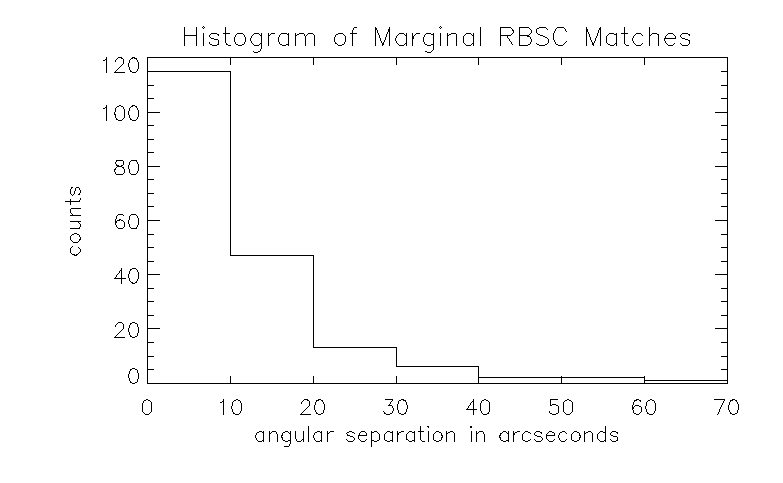
\includegraphics[height=6cm]{rass_histogram.eps}
	\label{xyz} 
\end{minipage}%
\begin{minipage}{.5\textwidth}
	\centering
	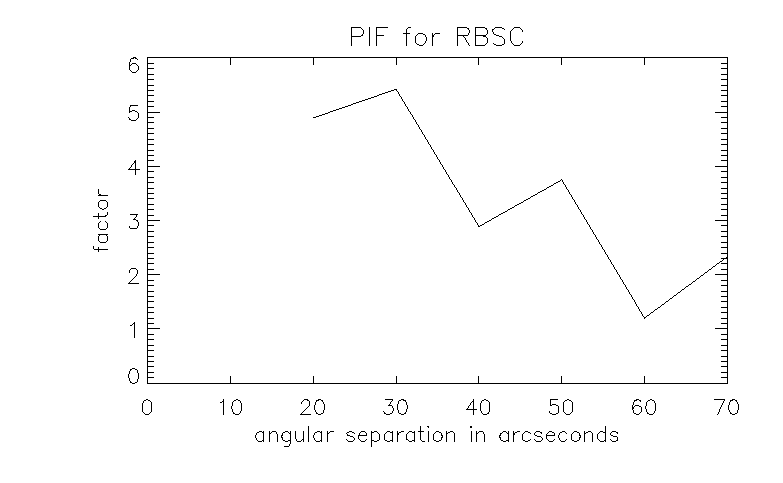
\includegraphics[height=6cm]{rass_factor.eps} 
	\label{xyz} 
\end{minipage}
\label{fig:test}
\end{figure} 

\begin{figure}[htbp] 
\hspace*{-0.55in}
\centering
\begin{minipage}{.5\textwidth}
	\centering
	\includegraphics[height=6cm]{CSC_histogram.eps}
	\label{xyz} 
\end{minipage}%
\begin{minipage}{.5\textwidth}
	\centering
	\includegraphics[height=6cm]{CSC_factor.eps} 
	\label{xyz} 
\end{minipage}
\label{fig:test}
\end{figure} 
\begin{multicols}{2}

For CSC, a similar histogram was formed for ranges a factor of ten smaller. A similar curve was seen, however the 1" to 2" annulus consisted of proportionally many more results than the 10" to 20" annulus as seen in the RBSC histogram. This suggests a slightly broader (scaled by ten) curve. PIF values were also calculated and graphed in the same manner as done for RBSC. The peak PIF value for CSC can be seen to be at or very close to 3". Because of the lack of enough data to analyze in the manner done by Voges or Parejko, and that this PIF peak has been shown to be a very agreeable distinction for RASS data, it was also selected to represent the CSC's precision in this circumstance. The CSC crossmatch radius has been chosen to be 3", which includes 89\% of all CSC matches within 7".

\subsubsection{Performing Crossmatches}\label{crossmatch}
\indent Now that both a maser control sample and a maser detection sample were available and angular radii were chosen, crossmatching could begin. Each item in the maser and control groups were matched by position to each catalog with various angular radii as previously determined.

The Sloan Digital Sky Survey (SDSS) has an vast collection of optical spectroscopic and photometric data collected from a 2.5 meter telescope in New Mexico at Apache Point University\cite{sdss}. The SDSS has an online catalog query system called casjobs that accepts SQL queries. A radius of 10" was used to compare the maser and control groups to SDSS Data Release 9 (DR9).

For the X-Ray catalogs a different approach was used. For Integral, Swift-BAT, XMM, RASS BSC and RASS FSC, the TOPCAT software was used. It had direct access to these catalogs and crossmatches were done completely with the software's pre-programmed angular radius crossmatching tool. For RASS we used 25", for Integral we used 20", and for Swift-BAT and 2XMMi-DR3 we used 10". For the Chandra Source Catalog, TOPCAT did not have direct access. As such, the crossmatches were run with CSC software in a similar manner, using an angular radius of 3". The results were then imported into TOPCAT to remove duplicates.

\section{Results}\label{results}
The first step in analyzing the newfound data was by calculating the detection rates. The maser and control group detection rates were calculated by dividing the number of detections in each group by the total size of each group. Then the ratio of maser detections to control group detections was calculated. The current below table is tentatively waiting on a 25" crossmatch of CSC, so an average of 20" and 30" results have been used temporarily as a place holder.

\end{multicols}
\begin {table}[h]
\caption {Detection Rates} \label{asdasd}
\begin{center}
{\footnotesize \begin{tabular} {|p{3cm}|p{1.2cm}|p{1.2cm}|p{0.8cm}|p{1.2cm}|p{1cm}|p{1cm}|p{1cm}|p{1cm}|p{1.2cm}|}
  \hline
Catalog & $E_L$ & $E_H$ & $E_m$ & Radius " & Control Count & Maser count & Control Rate & Maser rate & maser/ control \\
 \hline 
 \hline
RFSC ((20+30)/2) & 0.1 & 2 & 1.05 & 25 & 70 & 8.8 & 0.021 & 0.058 & 2.780 \\ \hline
RBSC ((20+30)/2) & 0.1 & 2 & 1.05 & 25 & 152.5 & 8.8 & 0.046 & 0.058 & 1.281 \\ \hline
CSC & 0.06 & 10 & 5.03 & 3 & 144 & 28 & 0.043 & 0.185 & 4.300 \\ \hline
2XMMi-DR3 & 0.2 & 12 & 6.1 & 10 & 294 & 52 & 0.088 & 0.344 & 3.911 \\ \hline
Swift-BAT 70 month & 14 & 150 & 82 & 10 & 191 & 34 & 0.057 & 0.225 & 3.936 \\ \hline
Integral & 15 & 10000 & 5007.5 & 20 & 14 & 5 & 0.004 & 0.033 & 7.897 \\ \hline
MEAN & & & & & & & 0.043 & 0.151 & 4.018 \\
  \hline
\end{tabular}}
\end{center}
\end {table}
\begin{multicols}{2}
The control detection rate was graphed against the maser detection rate, showing a clear correlation between the two. If a linear function is fit to this graph, the slope is found to be 4.157, close to the mean maser rate over control rate value of 4.018. A bar graph was then made depicting the maser over control value for each catalog, listing the catalogs in order of mean energy observed $E_m$. There was a clear correlation so each catalog's maser over control was plotted relative to the mean energy on a logarithmic scale. The correlation almost appears to fit to a line, which would represent a logarithmically fitting function if it actually is as simple as it appears at first glance.

[graphs are omitted because there is a problem getting idl working]

\section{Conclusions}\label{conclusion}
Format citations properly. Go back and talk about other catalogs: eg. the Swift-BAT chosen is the recent 70 month survey. Replace chart with appropriate detection values and add graphs. Ideally PIF would aid selection of radius for each catalog but time may be an issue. Filler was used for abstract and introduction to allow tables and graphs to fall into place nicely, as it is assumed there will be text there anyway and this more closely approximates a future appearance.
\end{multicols}


\begin{thebibliography}{1}
\bibitem{surv}
  \emph{MCP All-Surveyed List}.
  2013. \begin{verbatim}http://www.gb.nrao.edu/~jbraatz/H2O/sum_dir_sort.txt\end{verbatim} 
  
\bibitem{navigator}
  \emph{SDSS Navigator}.
  2013. \begin{verbatim} http://skyserver.sdss3.org/public/en/tools/chart/navi.asp\end{verbatim} 

\bibitem{sdss}
  \emph{Sloan Digital Sky Survey}.
  2013. \begin{verbatim} http://www.sdss.org/\end{verbatim} 
  
\bibitem{voges}
  \emph{The ROSAT all-sky survey bright source catalogue}.
  Astronomy and Astrophysics
  
\bibitem{parejko}
  \emph{SOURCE MATCHING IN THE SDSS AND RASS: WHICH GALAXIES ARE REALLY X-RAY SOURCES?}.
  The Astronomical Journal
  
  
\end{thebibliography}
\end{document}